% Included by sections/09-results.tex. Regenerate with
%   node workspace/figures/make_main_result_figure.mjs
% then copy workspace/figures/out/main_result.tex here and drop the standalone wrapper.
\begin{figure}[t]
\centering
\definecolor{vizA}{HTML}{2A78D6}
\definecolor{vizB}{HTML}{EB6834}
\definecolor{vizC}{HTML}{1BAF7A}
% Main result: solve rate per difficulty group.
% Generated by workspace/figures/make_main_result_figure.mjs
% Source: /Users/luxian/FoldOriganmi/workspace/RESULTS/results.md ("By model and tool tier")
% claude-sonnet-5 / tools=legal-folds: easy 0/5, medium --, hard --
% codex-cli-chatgpt / tools=none: easy 0/1, medium --, hard --
% deterministic-bfs / tools=legal-folds: easy 366/669, medium 1/40, hard 0/16
% gpt-5.6-luna / tools=legal-folds: easy 59/289, medium 0/66, hard 0/25
% gpt-5.6-luna / tools=none: easy 4/65, medium 0/1, hard 0/1
% gpt-5.6-sol / tools=none: easy 0/7, medium --, hard --
% gpt-5.6-terra / tools=none: easy 0/1, medium --, hard --
% gpt-6-astra / tools=none: easy 1/1, medium --, hard --
%
% Standalone: pdflatex main_result.tex
% In a paper: keep the tikzpicture, drop the documentclass wrapper.
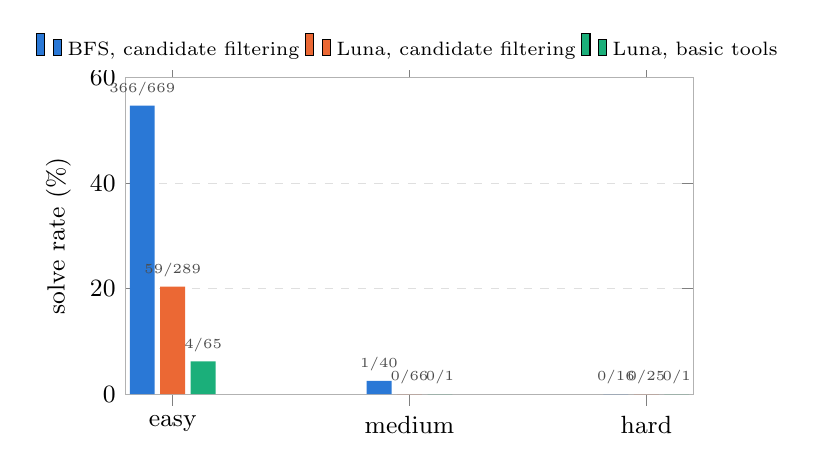
\begin{tikzpicture}
\begin{axis}[
  width=8.8cm, height=5.6cm,
  ybar, bar width=9pt,
  ymin=0, ymax=60,
  ylabel={solve rate (\%)},
  symbolic x coords={easy,medium,hard},
  xtick=data,
  point meta=explicit symbolic,
  nodes near coords={\pgfplotspointmeta},
  every node near coord/.append style={font=\tiny, color=black!70},
  tick label style={font=\small},
  label style={font=\small},
  legend style={font=\scriptsize, at={(0.5,1.16)}, anchor=north, legend columns=-1, draw=none},
  ymajorgrids, grid style={gray!25, dashed},
  axis line style={gray!60},
]
\addplot[fill=vizA, draw=none] coordinates {(easy,54.7) [366/669] (medium,2.5) [1/40] (hard,0.0) [0/16]};
\addlegendentry{BFS, candidate filtering}
\addplot[fill=vizB, draw=none] coordinates {(easy,20.4) [59/289] (medium,0.0) [0/66] (hard,0.0) [0/25]};
\addlegendentry{Luna, candidate filtering}
\addplot[fill=vizC, draw=none] coordinates {(easy,6.2) [4/65] (medium,0.0) [0/1] (hard,0.0) [0/1]};
\addlegendentry{Luna, basic tools}
\end{axis}
\end{tikzpicture}
\caption{\textbf{Solve rate by difficulty group.} Bars carry solved over attempts, and the
denominators are attempts rather than distinct samples, so one sample may be counted more
than once. The three arms shown are the ones with coverage enough to support a rate; the
five arms with fewer than ten attempts are omitted from the figure and account for 15
attempts, of which one was solved. Rates come from different sets of attempts and are not a
paired comparison on a matched sample set (Section~\ref{sec:results-threats}).}
\label{fig:main}
\end{figure}
